\begin{appendix}

\chapter{The SHA-256 Algorithm}
\label{app:hashing-algo}

The SHA-256 algorithm is a member of a set of algorithms referred to as the SHA-2 standard.
These are described in \cite{fips180-4} and consists of algorithms for producing hashes with
lengths of 224, 256, 384 and 512 bits.
The algorithms use simple operations, limited to shifts, rotates, xor, and unsigned additions,
common single-cycle operations for general purpose CPUs, in addition to a lookup-table of constants.
This allows for high-speed implementations in both software and hardware. The different SHA-2 algorithms
differ in how and with what parameters the various operations are invoked.

SHA-256 is the algorithm used in cryptocoin mining. It operates on blocks of 512~bits and keeps
a 256~bits long intermediate hash value as state. Bitcoin uses a double pass SHA-256 hash, which
first calculates the hash of a block of the data to be hashed and then hashes the hash of the first
pass.

Before the first block is processed, the initial hash value is set to a predefined
value. The entire message that is to be hashed is then padded by adding a 1~bit to
the end of the message and then appending zeroes until the length of the final block
is 448~bits. Then the length of the entire message, without padding, is added as a
64-bit big-endian integer to the end of the block.

Then, each input block is split into a 64 times 32-bit long expanded message block, where
each 32-bit word $W_j$ is defined according to the formula

\[ W_j = \left\{
	\begin{array}{l l}
		M_j & \quad j \in \left[0, 15\right]\\
		\sigma_1(W_{j - 2}) + W_{j - 7} + \sigma_0(W-{j - 15}) + W_{j - 15} & \quad j \in \left[16, 63\right]
	\end{array}
\right.\]

\noindent where $M_j$ is the $j$th word of the input message block and the functions
$\sigma_0$ and $\sigma_1$ are defined as

\[\sigma_0 = R^7(x) \oplus R^{18}(x) \oplus S^3(x)\]
\[\sigma_1 = R^{17}(x) \oplus R^{19}(x) \oplus S^{10}(x)\]

\noindent where the operator $R^n$ means right rotation by $n$ bits and $S^n$ means right shift by $n$
bits \footnote{Curiously, \cite{sha-spec} defines the operator $R$ as shift and $S$ as rotate.
We use the more intuitive definitions.}.

\subsubsection{The Compression Function}
\label{sec:sha-compr}
The compression function is the core of the SHA-256 algorithm. It uses a look-up table
of 64 constants, $K_j$, and the following functions when calculating the new intermediate
hash values:

\[Ch(x,y,z) = (x \wedge y) \oplus (\neg x \wedge z)\]
\[Maj(x, y, z) = (x \wedge y) \oplus (x \wedge z) \oplus (y \wedge z)\]
\[\Sigma_0(x) = R^2(x) \oplus R^{13}(x) \oplus R^{22}(x)\]
\[\Sigma_1(x) = R^6(x) \oplus R^{11}(x) \oplus R^{25}(x)\]

Before starting the iterations with the compression function, the intermediate
hash values from the previous message block are assigned to the variables $a$--$h$.

At the beginning of each iteration of the compression function, two temporary
values are calculated:

\[T_1 = h + \Sigma_1(e) + Ch(e, f, g) + K_j + W_j\]
\[T_2 = \Sigma_0(a) + Maj(a, b, c)\]

The new hash values are then assigned as follows:

\[\begin{array}{l}
	h \leftarrow g \\
	g \leftarrow f \\
	f \leftarrow e \\
	e \leftarrow d + T_1\\
	d \leftarrow c \\
	c \leftarrow b \\
	b \leftarrow a \\
	a \leftarrow T_1 + T_2 \\
\end{array}\]

The compression function is run 64 times, once for each word in the extended message block,
$W_j$. Afterwards, the intermediate hash for the message is updated by adding the
variables $a$--$h$ to the corresponding values of the intermediate hash values from
the previous message block.

When the final input block has been processed, the final hash is composed by
concatenating the intermediate hash values. \cite{sha-spec, fips180-4, fordypningsprosjekt}

\chapter{Additional Results}
\label{app:performance}

This chapter lists up all the details regarding the various measurements done during this thesis.
For each selected SHMAC architecture, the performance and power usage is measured for varying numbers
of active cores. Every architecture have been measured when running software-only hashing, when running
the SHA-256 accelerator without using the DMA module, and then with using the DMA module. 

\section{Performance Measurements}

\subsection{Initial Architecture}

The first architecture used for measuring, is the 5 by 4 grid architecture described in section \ref{sec:SHMAC_sys_arch}.
Unfortunately, while software hashing worked on all tiles, the application crashed when using the SHA-256 accelerator on more than one row
and was discarded. The reasons are discussed in section \ref{sec:init-results}.

The performance obtained when doing software hashing is listed in table \ref{tab:Full-Perf-SW1}. 

\begin{sidewaystable}
\centering
\begin{tabular}{| l || r r r r | r r r r | r r r | r r r r r |}
  \hline 
  \textbf{Sum} [H/s] & \textbf{0} & \textbf{1} & \textbf{2} & \textbf{3} & \textbf{4} & \textbf{5} & \textbf{6} & \textbf{7} & \textbf{8} & \textbf{9} & \textbf{10} & \textbf{11} & \textbf{12} & \textbf{13} & \textbf{14} & \textbf{15}   \\
  \hline                       
  \textbf{6450} & 6450 & - & - & - & - & - & - & - & - & - & - & - & - & - & - & - \\
  \textbf{12895} & 6446 &6449 & - & - & - & - & - & - & - & - & - & - & - & - & - & - \\
  \textbf{19190} & 6394 & 6398 & 6398 & - & - & - & - & - & - & - & - & - & - & - & - & - \\
  \textbf{21261} & 5312 & 5316 & 5316 & 5317 & - & - & - & - & - & - & - & - & - & - & - & - \\
  \textbf{19310} & 4085 & 4029 & 3191 & 3207 & 4798 & - & - & - & - & - & - & - & - & - & - & - \\
  \textbf{18388} & 3171 & 3154 & 2083 & 2090 & 3961 & 3929 & - & - & - & - & - & - & - & - & - & - \\
  \textbf{18265} & 2354 & 2349 & 1474 & 1474 & 3119 & 3120 & 4375 & - & - & - & - & - & - & - & - & - \\
  \textbf{18191} & 1964 & 1970 & 1143 & 1142 & 2993 & 2993 & 2993 & 2993 & - & - & - & - & - & - & - & -\\
  \textbf{18195} & 1455 & 1458 & 801 & 801 & 2239 & 2239 & 2240 & 2240 & 4722 & - & - & - & - & - & - & -\\
  \textbf{18192} & 1142 & 1146 & 630 & 629 & 1762 & 1762 & 1762 & 1762 & 3799 & 3798 & - & - & - & - & - & -\\
  \textbf{18194} & 820 & 823 & 440 & 439 & 1257 & 1257 & 1257 & 1256 & 3120 & 3119 & 4406 & - & - & - & - & -\\
  \textbf{18192} & 579 & 582 & 309 & 308 & 888 & 888 & 889 & 889 & 2572 & 2572 & 3887 & 3829 & - & - & - & -\\
  \textbf{18192} & 531 & 534 & 278 & 278 & 811 & 811 & 811 & 812 & 2417 & 2417 & 3745 & 2374 & 2373 & - & - & -\\
  \textbf{18191} & 528 & 531 & 278 & 279 & 809 & 809 & 808 & 809 & 2411 & 2411 & 3737 & 1324 & 1324 & 2133 & - & -\\
  \textbf{18191} & 528 & 531 & 276 & 277 & 807 & 807 & 807 & 806 & 2406 & 2406 & 3730 & 875 & 875 & 1541 & 1519	 & -\\
  \textbf{18191} & 528 & 530 & 276 & 276 & 806 & 805 & 806 & 805 & 2402 & 2402 & 3723 & 827 & 828 & 1490 & 844 & 843\\
  \hline  
\end{tabular}
\caption{Software performance, for an increasing number of cores active.}
\label{tab:Full-Perf-SW1}
\end{sidewaystable}

Tables \ref{tab:Perf-SHA1} and \ref{tab:Perf-SHADMA1} show the results when using the SHA-256 hashing accelerator, without and with DMA module, respectively.
Only four cores were used because of the scratchpad bug mentioned in section \ref{sec:init-results}.

%The linear increase and the comparison between the two can be seen in the plots of figure \ref{fig:shadmacomp-scaling1}.

\begin{table}
\centering
\begin{tabular}{| l || r r r r |}
  \hline 
  \textbf{Sum} [H/s] & \textbf{0} & \textbf{1} & \textbf{2} & \textbf{3}\\
  \hline                       
  \textbf{17557} & 17557 & - & - & - \\
  \textbf{37539} & 17528 & 20011 & - & - \\
  \textbf{54912} & 17481 & 19941 & 17490 & - \\
  \textbf{70179} & 17400 & 19891 & 17411 & 15477 \\
  \hline  
\end{tabular}
\caption{Performance when using the SHA-256 accelerator only in the initial architecture.}
\label{tab:Perf-SHA1}
\end{table}


\begin{table}
\centering
\begin{tabular}{| l || r r r r |}
  \hline 
  \textbf{Sum} [H/s] & \textbf{0} & \textbf{1} & \textbf{2} & \textbf{3}\\
  \hline                       
  \textbf{18230} & 18230 & - & - & - \\
  \textbf{38267} & 18189 & 20078 & - & - \\
  \textbf{56150} & 18129 & 19880 & 18141 & - \\
  \textbf{71840} & 17973 & 19577 & 17984 & 16306 \\
  \hline  
\end{tabular}
\caption{Performance when using the SHA-256 accelerator and DMA in the initial architecture.}
\label{tab:Perf-SHADMA1}
\end{table}
		
%\subsection{Comparison, 5x4}
%
%The difference between software hashing and use of accelerator with DMA are compared in figure \ref{fig:comp-plot1}, where software hashing is seen in red plot, and accelerator hashing is seen in black plot.
%As seen in the figure, the hashing modules greatly outperforms the software hashing, even with only up to four processors in use.
%
%\begin{figure}
%	\begin{tikzpicture}
%		\begin{axis}[
%			xlabel=Active processor tiles,
%			ylabel=Sum of hashes/S]
%		\addplot[color=red,mark=x] coordinates {
%			(1, 6450)
%			(2, 12895)
%			(3, 19190)
%			(4, 21261)
%			(5, 19310)
%			(6, 18388)
%			(7, 18265)
%			(8, 18191)
%			(9, 18195)
%			(10, 18192)
%			(11, 18194)
%			(12, 18192)
%			(13, 18192)
%			(14, 18191)
%			(15, 18191)
%			(16, 18191)
%		};
%		\addplot[color=black,mark=o] coordinates {
%			(1, 18230)
%			(2, 38267)
%			(3, 56150)
%			(4, 71840)
%		};
%		\end{axis}
%	\end{tikzpicture}
%	\caption{Sum of double hashes per second. Red: Software only, Black: SHA-256 + DMA, 5x4 architecture}
%	\label{fig:comp-plot1}
%\end{figure}

\subsection{Alternative Architecture}

%Since the scratchpad-bug prevents us from measuring more than one tile row, a different architecture has been synthesized and tested, as seen in figure \ref{fig:15x2-2}.
%This one circumwents the scratchpad-but by having all CPU tiles on the same upper row, while filling the second with BRAM, DDR-RAM and empty tiles only.
%This way, the use of more tiles may be measured, with the interest to find a possible congestion limit when using SHA-256 accelerator.
%15 tiles per row (or more likely, 14 CPU tiles on upper row) was the maximum number, allowed by the compiler.
%It is likely that the interconnect network may become congested earlier than in a different architecture, due to the XY-routing, given that the all CPU-tiles will be competing for the network on the upper row, while the lower row is almost unused.
%
%\begin{figure}[htb]
%    \centering
%    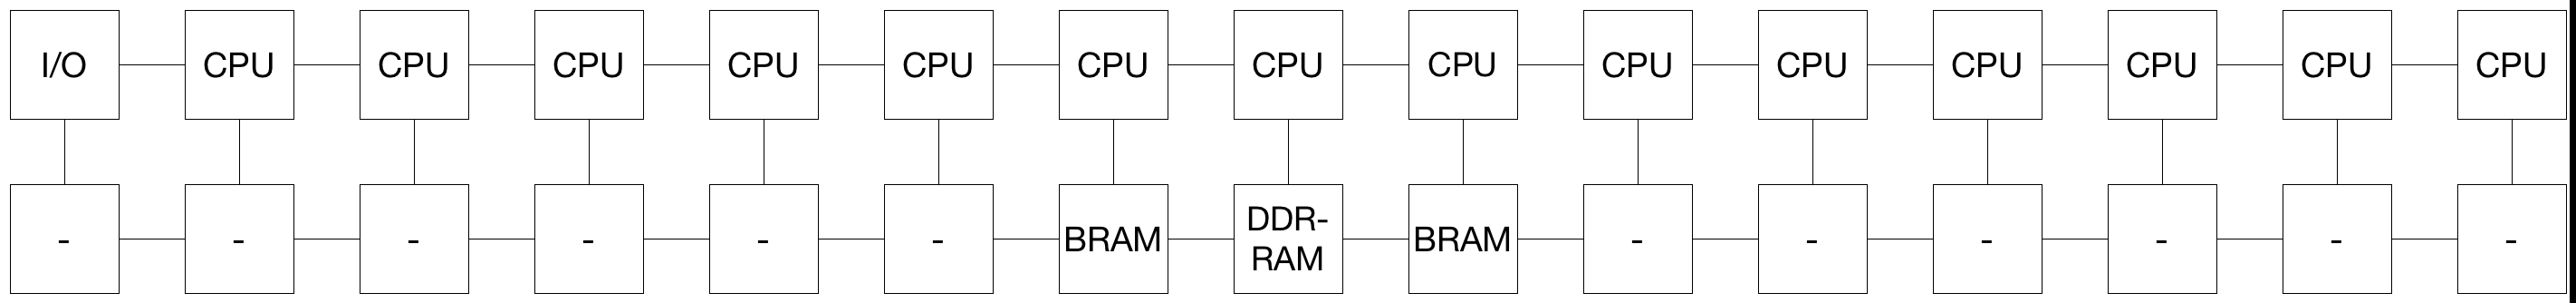
\includegraphics[width=1.0\textwidth]{Figures/Measurements/15x2}
%    \caption{Test setup 2, with BRAM and DDR-RAM tiles on second row, and all CPU's and I/O on the first row.}
%    \label{fig:15x2-2}
%\end{figure}
%

The results from doing the software hashing for this architecture is listed in table \ref{tab:Full-Perf-SW2}. 
The CPU tiles nearest the DRAM tile have highest individual performance compared to others present.
%The plot in figure \ref{fig:sw-scaling2APP} confirms that the pattern is the same: The application does not improve beyond four active tiles.
%Once again, congested memory is the reason.

\begin{sidewaystable}
\centering
\begin{tabular}{| l || r r r r r r r r r r r r r r|}
  \hline 
  \textbf{Sum} [H/s] & \textbf{0} & \textbf{1} & \textbf{2} & \textbf{3} & \textbf{4} & \textbf{5} & \textbf{6} & \textbf{7} & \textbf{8} & \textbf{9} & \textbf{10} & \textbf{11} & \textbf{12} & \textbf{13}\\
  \hline                       
  \textbf{6418} & 6418 & - & - & - & - & - & - & - & - & - & - & - & - & -\\
  \textbf{12841} & 6419 & 6422 & - & - & - & - & - & - & - & - & - & - & - & -\\
  \textbf{19130} & 6374 & 6378 & 6378 & - & - & - & - & - & - & - & - & - & - & -\\
  \textbf{21364} & 5338 & 5342 & 5342 & 5342 & - & - & - & - & - & - & - & - & - & -\\
  \textbf{19404} & 3186 & 3158 & 3883 & 4471 & 4706 & - & - & - & - & - & - & - & - & -\\
  \textbf{18420} & 1723 & 1718 & 2538 & 3506 & 4313 & 4622 & - & - & - & - & - & - & - & -\\
  \textbf{18253} & 945 & 944 & 1549 & 2410 & 3472 & 4304 & 4629 & - & - & - & - & - & - & -\\
  \textbf{18206} & 516 & 519 & 902 & 1532 & 2442 & 3505 & 4358 & 4432 & - & - & - & - & - & -\\
  \textbf{18193} & 345 & 348 & 633 & 1139 & 1958 & 3102 & 4257 & 3240 & 3171 & - & - & - & - & -\\
  \textbf{18192} & 313 & 315 & 582 & 1057 & 1834 & 2997 & 4231 & 3017 & 1969 & 1877 & - & - & - & -\\
  \textbf{18192} & 311 & 312 & 573 & 1040 & 1821 & 2979 & 4221 & 2989 & 1823 & 1096 & 1027 & - & - & -\\
  \textbf{18192} & 308 & 310 & 570 & 1032 & 1818 & 2970 & 4217 & 2980 & 1819 & 1036 & 587 & 545 & - & -\\
  \textbf{18191} & 307 & 309 & 571 & 1032 & 1811 & 2965 & 4216 & 2974 & 1810 & 1035 & 565 & 305 & 291 & -\\
  \textbf{18190} & 307 &310 & 570 & 1030 & 1809 & 2962 & 4211 & 2971 & 1809 & 1034 & 564 & 298 & 158 & 157\\
  \hline  
\end{tabular}
\caption{Software performance results for the alternative architecture.}
\label{tab:Full-Perf-SW2}
\end{sidewaystable}

Tables \ref{tab:Perf-SHA2} and \ref{tab:Perf-SHADMA2} show the results when using the SHA-256 accelerator in the alternative architecture, without and with DMA module, respectively.
This time, using an architecture that circumvents the cache-bug problem, all available CPUs are used in the tests.

%The trend is the same, with a near-linear increase.
%It may be observed from the table results that the closer a specific tile is in proximity to the BRAM-tiles, the higher the individual performance, with highest performance observed at CPU tiles 4-6.
%This counts for both without and with DMA. 
%The plots in figure \ref{fig:shadmacomp-scaling2} seems to confirm this trend: The increase become greater as the processors closer to the middle become active, and lessens beyond that point.
%It also seems that the increase when adding the final tiles are less, compared to when adding the first tiles from left, indicating that the system is reaching a saturation point.
%However, there were not enough CPU-tiles available for reaching maximum performance.
%
%An interesting observation, seen in the tables, is that as more tiles are added, the gain from using the DMA is reduced per tile.
%As all CPU tiles become active, CPU tiles 0-6 shows less performace compared to not using DMA, with CPU tile 5 having the biggest drop of nearly 4000 double hashes. 
%CPU tiles 6-11 shows a steady increase per tile, but only up to around 500 double hashes per second.
%The total performance loss becomes so negative that after adding the 13th CPU tile, omitting the DMA module actually increases the performance.
%This is seen in figure \ref{fig:shadmacomp-scaling2}-
%
%Judging from the positions in figure \ref{fig:15x2-2APP}It seems that the closer a CPU tile is to the  BRAM-tiles from left, the more negative the use of DMA is.
%
%The cause is likely the 32-bit data transfers by the DMA module on all tiles.
%For each 128-bit block, the DMA Module must do four individual transfers, requesting data from the same block four times over.
%While a single DMA Module cleary performs better than a Turbo Amber CPU, the collective number of DMA transfers must be causing the interconnect network to saturate much faster, reaching a point where the performance gain is lowered much faster.

\begin{sidewaystable}
\centering
\begin{tabular}{| l || r r r r r r r r r r r r r r |}
  \hline 
  \textbf{Sum} [H/s] & \textbf{0} & \textbf{1} & \textbf{2} & \textbf{3} & \textbf{4} & \textbf{5} & \textbf{6} & \textbf{7} & \textbf{8} & \textbf{9} & \textbf{10} & \textbf{11} & \textbf{12} & \textbf{13}\\
  \hline                       
  \textbf{11676} & 11676 & - & - & - & - & - & - & - & - & - & - & - & - & -\\
  \textbf{24394} & 11664 & 12730 & - & - & - & - & - & - & - & - & - & - & - & -\\
  \textbf{38329} & 11642 & 12699 & 13988 & - & - & - & - & - & - & - & - & - & - & -\\
  \textbf{53760} & 11618 & 12660 & 13951 & 15531 & - & - & - & - & - & - & - & - & - & -\\
  \textbf{70983} & 11563 & 12600 & 13872 & 15463 & 17485 & - & - & - & - & - & - & - & - & -\\
  \textbf{90590} & 11503 & 12533 & 13800 & 15371 & 17384 & 19999 & - & - & - & - & - & - & - & -\\
  \textbf{107510} & 11438 & 12454 & 13711 & 15270 & 17265 & 19897 & 17475 & - & - & - & - & - & - & -\\
  \textbf{122186} & 11366 & 12372 & 13621 & 15163 & 17136 & 19779 & 17339 & 15410 & - & - & - & - & - & -\\
  \textbf{135009} & 11295 & 12299 & 13527 & 15046 & 17001 & 19663 & 17195 & 15261 & 13722 & - & - & - & - & -\\
  \textbf{146221} & 11222 & 12212 & 13423 & 14918 & 16855 & 19546 & 17029 & 15104 & 13574 & 12338 & - & - & - & -\\
  \textbf{156133} & 11140 & 12123 & 13320 & 14794 & 16722 & 19431 & 16852 & 14931 & 13418 & 12200 & 11202 & - & - & -\\
  \textbf{164860} & 11068 & 12038 & 13225 & 14675 & 16585 & 19319 & 16653 & 14741 & 13234 & 12041 & 11056 & 10225 & - & -\\
  \textbf{172381} & 10988 & 11943 & 13109 & 14541 & 16422 & 19208 & 16422 & 14538 & 13028 & 11844 & 10882 & 10070 & 9386 & -\\
  \textbf{179526} & 10944 & 11891 & 13045 & 14461 & 16329 & 19123 & 16306 & 14347 & 12839 & 11669 & 10721 & 9925 & 9253 & 8673 \\
  \hline  
\end{tabular}
\caption{Performance results when using the SHA-256 accelerator in the alternative architecture.}
\label{tab:Perf-SHA2}
\end{sidewaystable}

\begin{sidewaystable}
\centering
\begin{tabular}{| l || r r r r r r r r r r r r r r |}
  \hline 
  \textbf{Sum} [H/s] & \textbf{0} & \textbf{1} & \textbf{2} & \textbf{3} & \textbf{4} & \textbf{5} & \textbf{6} & \textbf{7} & \textbf{8} & \textbf{9} & \textbf{10} & \textbf{11} & \textbf{12} & \textbf{13}\\
  \hline                       
  \textbf{13227} & 13227 & - & - & - & - & - & - & - & - & - & - & - & - & -\\
  \textbf{27410} & 13220 & 14190 & - & - & - & - & - & - & - & - & - & - & - & -\\
  \textbf{42627} & 13183 & 14157 & 15287 & - & - & - & - & - & - & - & - & - & - & -\\
  \textbf{58989} & 13124 & 14091 & 15218 & 16556 & - & - & - & - & - & - & - & - & - & -\\
  \textbf{76556} & 13027 & 13991 & 15102 & 16431 & 18005 & - & - & - & - & - & - & - & - & -\\
  \textbf{95259} & 12869 & 13828 & 14920 & 16213 & 17769 & 19660 & - & - & - & - & - & - & - & -\\
  \textbf{112599} & 12695 & 13621 & 14691 & 15961 & 17495 & 19307 & 18829 & - & - & - & - & - & - & -\\
  \textbf{127515} & 12487 & 13393 & 14443 & 15689 & 17145 & 18885 & 18568 & 16905 & - & - & - & - & - & -\\
  \textbf{139937} & 12231 & 13085 & 14115 & 15326 & 16762 & 18411 & 18225 & 16597 & 15185 & - & - & - & - & -\\
  \textbf{150069} & 11911 & 12749 & 13783 & 14959 & 16333 & 17862 & 17749 & 16176 & 14867 & 13680 & - & - & - & -\\
  \textbf{158421} & 11585 & 12456 & 13402 & 14560 & 15971 & 17278 & 17236 & 15782 & 14441 & 13323 & 12387 & - & - & -\\
  \textbf{165271} & 11291 & 12094 & 13039 & 14193 & 15685 & 16642 & 16627 & 15491 & 14055 & 12927 & 12007 & 11220 & - & -\\
  \textbf{171143} & 10967 & 11768 & 12720 & 13935 & 15445 & 15971 & 15965 & 15290 & 13829 & 12619 & 11679 & 10900 & 10055 & -\\
  \textbf{175711} & 10625 & 11447 & 12461 & 13803 & 15040 & 15282 & 15274 & 14942 & 13676 & 12374 & 11375 & 10559 & 9726 & 9127\\
  \hline  
\end{tabular}
\caption{Performance results when using the SHA-256 accelerator with DMA in the alternative architecture.}
\label{tab:Perf-SHADMA2}
\end{sidewaystable}

%\subsection{Comparison, 15x2}
%
%The difference between software hashing and use of accelerator with omitting the DMA (as this gives best performance in the end) are compared in figure \ref{fig:comp-plot2}, where software hashing is seen in red plot, and accelerator hashing is seen in black plot.
%As seen in the figure, the hashing modules greatly outperforms the software hashing by far.
%
%\begin{figure}
%	\begin{tikzpicture}
%		\begin{axis}[
%			xlabel=Active processor tiles,
%			ylabel=Sum of double hashes/S]
%		\addplot[color=red,mark=x] coordinates {
%			(1, 6418)
%			(2, 12841)
%			(3, 19130)
%			(4, 21364)
%			(5, 19404)
%			(6, 18420)
%			(7, 18253)
%			(8, 18206)
%			(9, 18193)
%			(10, 18192)
%			(11, 18192)
%			(12, 18192)
%			(13, 18191)
%			(14, 18190)
%		};
%		\addplot[color=black,mark=o] coordinates {
%			(1, 11676)
%			(2, 24394)
%			(3, 38329)
%			(4, 53760)
%			(5, 70983)
%			(6, 90590)
%			(7, 107510)
%			(8, 122186)
%			(9, 135009)
%			(10, 146221)
%			(11, 156133)
%			(12, 164860)
%			(13, 172381)
%			(14, 179526)
%		};
%		\end{axis}
%	\end{tikzpicture}
%	\caption{Sum of hashes per second. Red: Software only, Black: SHA-256 (no DMA), 15x2 architecture}
%	\label{fig:comp-plot2}
%\end{figure}

\section{Power measurements}

%\section{Methodology}
%
%For a chosen architecture, and for a set of active CPU's, the power was measured along with performance.
%It turned out that it constantly fluctuated, and therefore we have chosen the average based on observations of highest and lower power consumption observed.
%The average power consumption together with uncertainty per measurement are filled into the tables in this chapter, and for each power consumption number, the power usage of the application is calculated.
%Calculated power usage is then plotted into graphs, with the uncertainty omitted. 
%
%The smallest unit we could measure in was 0.1 W. 

%It should be noted that the power changed somewhat over time. For instance, after measuring every tile configuration on the 15x2 architecture using the SHA-256 module with DMA, turning the number of active CPU tiles back to 1 showed an increase in average power of 0.3 W.
%This highligts the potential uncertainty about the test.
%Causes can be due to the environment (for instance, room temperature) or the system in Versatile Express that we have no control over.
%
%Due to the changing power consumption, we have constantly measured idle power between each individual test, and idle power used for calculations is based on the average from measuring first tile to all tiles in a set architecture and \todo{Kristian will add "Makes no sense" to this sentence. Improve later}configuration.
%
%\section{5x4 Architecture}
%
%\subsection{Software hashing power consumption, 5x4 Architecture.}

\subsection{Energy Efficiency for the Initial Test Setup}
\label{sec:energy-initial}

Table \ref{tab:SW-power1} shows the measured power usage, along with uncertainty and calculated application power of the initial test architecture.
The data is plotted in figure \ref{fig:SW-power1}.
%It appears that the more tiles are active, the less power is consumed by the system.
%On reason for this may be that as more tiles are added, longer periods of stalling is needed for each core to wait for data from the main memory.
%When cores are inactive, they are waiting in a nop-operation loop, a software loop consisting of a \textsc{nop} operation.
%Executing this loop causes the processor to have to decode and execute two instructions, the no-operation instruction
%and the branch instruction. However, when stalling, the processor does not decode or execute new instructions,
%which may cause less switching to happen internally in the processor.

\begin{table}
\centering
\begin{tabular}{| l | r | r || r |}
  \hline 
  \textbf{Cores} & \textbf{Average System Power [W]} & \textbf{Uncertainty} & \textbf{Application Power [W]} \\
  \hline                       
  \textbf{Idle} &  34.3 & 0.4 & 0.0\\
  \textbf{1} &  36.6 & 0.4 & 2.3\\
  \textbf{2} &  36.7 & 0.3 & 2.4\\
  \textbf{3} &  36.7 & 0.4 & 2.4\\
  \textbf{4} &  35.3 & 0.4 & 1.0\\
  \textbf{5} &  35.0 & 0.2 & 0.7\\
  \textbf{6} &  35.1 & 0.3 & 0.8\\
  \textbf{7} &  35.0 & 0.2 & 0.7\\
  \textbf{8} &  34.9 & 0.3 & 0.6\\
  \textbf{9} &  34.9 & 0.2 & 0.6\\
  \textbf{10} &  34.9 & 0.3 & 0.6\\
  \textbf{11} &  34.9 & 0.3 & 0.6\\
  \textbf{12} &  34.8 & 0.2 & 0.5\\
  \textbf{13} &  34.9 & 0.3 & 0.6\\
  \textbf{14} &  34.9 & 0.4 & 0.6\\
  \textbf{15} &  35.0 & 0.4 & 0.7\\
  \textbf{16} &  34.8 & 0.2 & 0.5\\
  \hline 
\end{tabular}
\caption{Measured power usage for software hashing using the initial test architecture.}
\label{tab:SW-power1}
\end{table}

\begin{figure}
\centering
	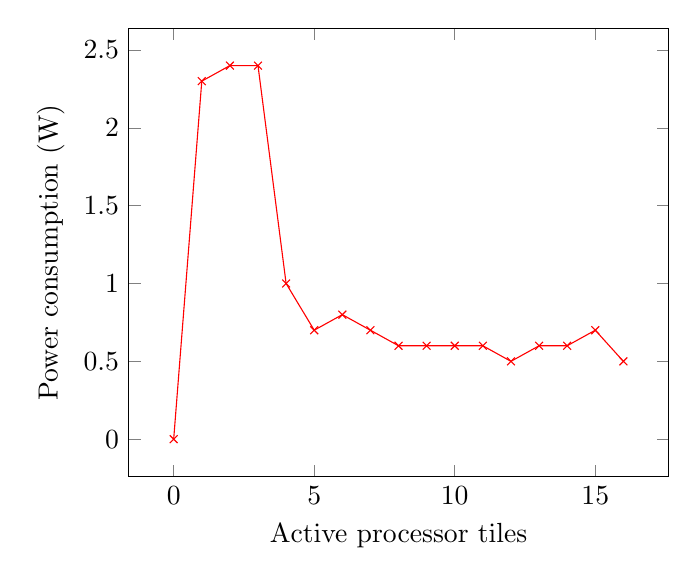
\begin{tikzpicture}
		\begin{axis}[
			xlabel=Active processor tiles,
			ylabel=Power consumption (W),
			scaled ticks=false]
		\addplot[color=red,mark=x] coordinates {
			(0, 0.0)
			(1, 2.3)
			(2, 2.4)
			(3, 2.4)
			(4, 1.0)
			(5, 0.7)
			(6, 0.8)
			(7, 0.7)
			(8, 0.6)
			(9, 0.6)
			(10, 0.6)
			(11, 0.6)
			(12, 0.5)
			(13, 0.6)
			(14, 0.6)
			(15, 0.7)
			(16, 0.5)
			
		};
		\end{axis}
	\end{tikzpicture}
	\caption{Measured power consumption for software hashing using the initial test architecture.}
	\label{fig:SW-power1}
\end{figure}

Tables \ref{tab:SHA-power1} and \ref{tab:SHADMA-power1} shows the individual power usage measured when using the SHA-256 accelerator without and with DMA module, respectively. 
Uncertainty and calculated application power is included as well. The data are plotted in figures \ref{fig:SHA-power1}.
As can be seen from the tables and figure, there is no significant difference in power usage when running with and without the DMA.

\begin{table}
\centering
\begin{tabular}{| l | r | r || r |}
  \hline 
  \textbf{Cores} & \textbf{Average System Power [W]} & \textbf{Uncertainty} & \textbf{Application Power [W]} \\
  \hline                       
  \textbf{Idle} &  34.3 & 0.4 & 0.0 \\
  \textbf{1} &  36.5 & 0.5 & 2.2\\
  \textbf{2} &  36.5 & 0.5 & 2.2\\
  \textbf{3} &  36.3 & 0.4 & 2.0\\
  \textbf{4} &  36.4 & 0.4 & 2.1\\
  \hline 
\end{tabular}
\caption{Power usage using the SHA-256 accelerator using the initial test architecture.}
\label{tab:SHA-power1}
\end{table}

\begin{table}
\centering
\begin{tabular}{| l | r | r || r |}
  \hline 
  \textbf{Cores} & \textbf{Average System Power [W]} & \textbf{Uncertainty} & \textbf{Application Power [W]} \\
  \hline                          
  \textbf{Idle} &  34.3 & 0.4 & 0.0 \\
  \textbf{1} &  36.4 & 0.4 & 2.1\\
  \textbf{2} &  36.7 & 0.3 & 2.3\\
  \textbf{3} &  36.6 & 0.4 & 2.2\\
  \textbf{4} &  36.6 & 0.4 & 2.2\\
  \hline 
\end{tabular}
\caption{Power usage using the SHA-256 accelerator and DMA using the initial test architecture.}
\label{tab:SHADMA-power1}
\end{table}

\begin{figure}
\centering
	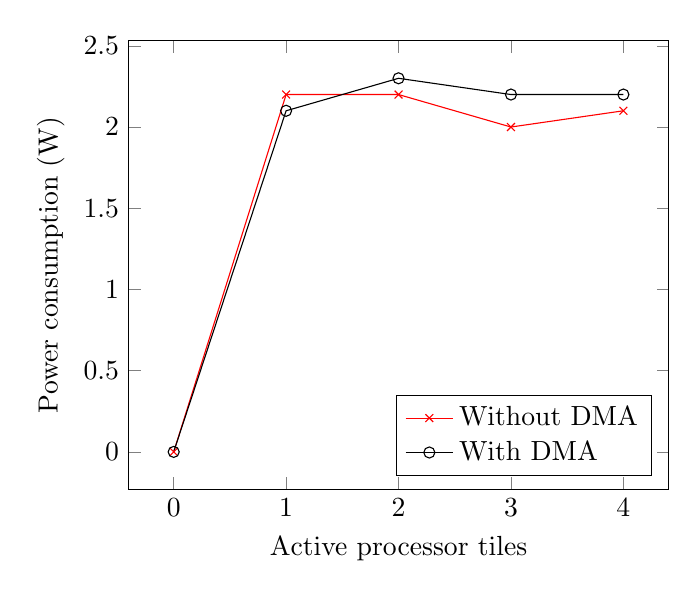
\begin{tikzpicture}
		\begin{axis}[
			xlabel=Active processor tiles,
			ylabel=Power consumption (W),
			scaled ticks=false,
			legend pos=south east,
			legend cell align=left]
		\addplot[color=red,mark=x] coordinates {
			(0, 0)
			(1, 2.2)
			(2, 2.2)
			(3, 2.0)
			(4, 2.1)
		};
		\addlegendentry{Without DMA}
		\addplot[color=black,mark=o] coordinates {
			(0, 0)
			(1, 2.1)
			(2, 2.3)
			(3, 2.2)
			(4, 2.2)
		};
		\addlegendentry{With DMA}
		\end{axis}
	\end{tikzpicture}
	\caption{Calculated power consumption using hardware accelerators}
	\label{fig:SHA-power1}
\end{figure}

\subsection{Alternative Architecture}

Table \ref{tab:SW-power2} shows the power measurements for the alternative architecture.

\begin{table}
\centering
\begin{tabular}{| l | r | r || r |}
  \hline 
  \textbf{Cores} & \textbf{Average System Power [W]} & \textbf{Uncertainty} & \textbf{Application Power [W]} \\
  \hline                         
  \textbf{Idle} & 33.9 & 0.3 & 0.0\\
  \textbf{1} & 36.2 & 0.3 & 2.3\\
  \textbf{2} & 36.4 & 0.4 & 2.5\\
  \textbf{3} & 36.2 & 0.4 & 2.3\\
  \textbf{4} & 34.9 & 0.3 & 1.0\\
  \textbf{5} & 34.8 & 0.2 & 0.9\\
  \textbf{6} & 34.7 & 0.3 & 0.8\\
  \textbf{7} & 34.7 & 0.3 & 0.8\\
  \textbf{8} & 34.7 & 0.3 & 0.8\\
  \textbf{9} & 34.6 & 0.4 & 0.7\\
  \textbf{10} & 34.6 & 0.4 & 0.7\\
  \textbf{11} & 34.7 & 0.3 & 0.8\\
  \textbf{12} & 34.7 & 0.3 & 0.8\\
  \textbf{13} & 34.6 & 0.4 & 0.7\\
  \textbf{14} & 34.6 & 0.4 & 0.7\\
  \hline 
\end{tabular}
\caption{Measured power usage when doing software hashing in the alternative architecture.}
\label{tab:SW-power2}
\end{table}

Tables \ref{tab:SHA-power2} and \ref{tab:SHADMA-power2} shows the individual power usage when using the SHA-256 accelerator without and with DMA module, respectively. 
Uncertainty and calculated application power are included as well.

\begin{table}
\centering
\begin{tabular}{| l | r | r || r |}
  \hline 
  \textbf{Cores} & \textbf{Average System Power [W]} & \textbf{Uncertainty} & \textbf{Application Power [W]} \\
  \hline                           
  \textbf{Idle} & 33.8 & 0.3 & 0.0\\
  \textbf{1} & 35.9 & 0.3 & 2.1\\
  \textbf{2} & 35.9 & 0.3 & 2.1\\
  \textbf{3} & 35.9 & 0.3 & 2.1\\
  \textbf{4} & 35.9 & 0.3 & 2.1\\
  \textbf{5} & 35.9 & 0.3 & 2.1\\
  \textbf{6} & 35.9 & 0.3 & 2.1\\
  \textbf{7} & 35.8 & 0.3 & 2.0\\
  \textbf{8} & 35.7 & 0.4 & 1.9\\
  \textbf{9} & 35.6 & 0.4 & 1.8\\
  \textbf{10} & 35.4 & 0.4 & 1.6\\
  \textbf{11} & 35.4 & 0.3 & 1.6\\
  \textbf{12} & 35.3 & 0.4 & 1.5\\
  \textbf{13} & 35.1 & 0.3 & 1.3\\
  \textbf{14} & 34.9 & 0.3 & 1.1\\
  \hline 
\end{tabular}
\caption{Measured power usage when using the SHA-256 accelerator without the DMA in the alternative architecture.}
\label{tab:SHA-power2}
\end{table}

\begin{table}
\centering
\begin{tabular}{| l | r | r || r |}
  \hline 
  \textbf{Cores} & \textbf{Average System Power [W]} & \textbf{Uncertainty} & \textbf{Application Power [W]} \\
  \hline                       
  \textbf{Idle} &  33.8 & 0.3 & 0.0\\
  \textbf{1} &  36.0 & 0.3 & 2.2\\
  \textbf{2} &  36.2 & 0.3 & 2.4\\
  \textbf{3} &  36.1 & 0.4 & 2.3\\
  \textbf{4} &  36.2 & 0.3 & 2.4\\
  \textbf{5} &  36.2 & 0.3 & 2.4\\
  \textbf{6} &  36.2 & 0.3 & 2.4\\
  \textbf{7} &  36.1 & 0.3 & 2.3\\
  \textbf{8} &  36.0 & 0.3 & 2.2\\
  \textbf{9} &  35.7 & 0.3 & 1.9\\
  \textbf{10} &  35.8 & 0.3 & 2.0\\
  \textbf{11} &  35.7 & 0.3 & 1.9\\
  \textbf{12} &  35.8 & 0.2 & 2.0\\
  \textbf{13} &  35.7 & 0.4 & 1.9\\
  \textbf{14} &  35.5 & 0.4 & 1.7\\
  \hline 
\end{tabular}
\caption{Measured power usage when using the SHA-256 accelerator with DMA in the alternative architecture.}
\label{tab:SHADMA-power2}
\end{table}

\section{Energy Efficiency}

In this chapter, the energy efficiency is presented, calculated from the measured performance and energy usage.

\subsection{Initial Architecture}

The energy efficiency of software hashing in the initial architecture can be seen in table \ref{tab:SW-eff1}, and the corresponding plot in figure \ref{fig:SW-eff1}.

\begin{table}
\centering
\begin{tabular}{| l | r | r || r |}
  \hline 
  \textbf{Cores} & \textbf{H/s} & \textbf{W} & \textbf{H/s/W} \\
  \hline                       
  \textbf{1} &  6450 & 2.3 & 2804.3\\
  \textbf{2} &  12895 & 2.4 & 5372.9\\
  \textbf{3} &  19190 & 2.4 & 7995.8\\
  \textbf{4} &  21261 & 1.0 & 21261\\
  \textbf{5} &  19310 & 0.7 & 27585.7\\
  \textbf{6} &  18388 & 0.8 & 22985\\
  \textbf{7} &  18265 & 0.7 & 26092.9\\
  \textbf{8} &  18191 & 0.6 & 30318.3\\
  \textbf{9} &  18195 & 0.6 & 30325\\
  \textbf{10} &  18192 & 0.6 & 30320\\
  \textbf{11} &  18194 & 0.6 & 30323.3\\
  \textbf{12} &  18192 & 0.5 & 36384\\
  \textbf{13} &  18192 & 0.6 & 30320\\
  \textbf{14} &  18191 & 0.6 & 30318.3\\
  \textbf{15} &  18191 & 0.7 & 25987,1\\
  \textbf{16} &  18191 & 0.5 & 36382\\
  \hline 
\end{tabular}
\caption{Energy efficiency of software hashing in the initial architecture.}
\label{tab:SW-eff1}
\end{table}

\begin{figure}
\centering
	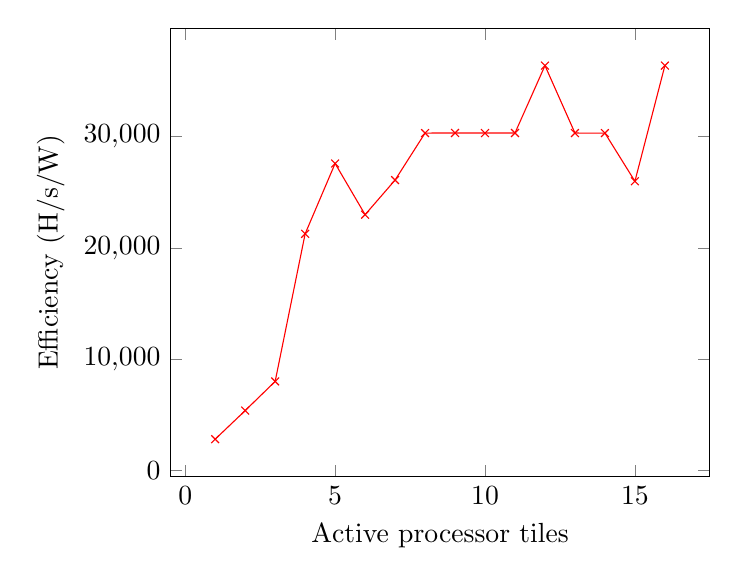
\begin{tikzpicture}
		\begin{axis}[
			xlabel=Active processor tiles,
			ylabel=Efficiency (H/s/W),
			scaled ticks=false]
		\addplot[color=red,mark=x] coordinates {
			(1, 2804.3)
			(2, 5372.9)
			(3, 7995.8)
			(4, 21261)
			(5, 27585.7)
			(6, 22985)
			(7, 26092.9)
			(8, 30318.3)
			(9, 30325)
			(10, 30320)
			(11, 30323.3)
			(12, 36384)
			(13, 30320)
			(14, 30318.3)
			(15, 25987.1)
			(16, 36382)
		};
		\end{axis}
	\end{tikzpicture}
	\caption{Energy efficiency of software hashing in the initial architecture.}
	\label{fig:SW-eff1}
\end{figure}

Tables \ref{tab:SHA-eff1} and \ref{tab:SHADMA-eff1} shows the energy efficiency of the SHA-256 accelerator, without and with using the DMA module, respectively.
The plot for both can be seen in figure \ref{fig:SHADMA-eff1}, where they are compared to each other.

%While using the DMA in the start is slightly more efficient, it drops below omitting it when 2 or more tiles are active.
%The performance is slightly higher, but so is the energy consumption, if only with few mere units of '0.1 W's.
%This implies the very sensitivity due to the uncertainty around measuring the fluctuating power from the wall.
%
%It is known from measuring power usage in section \label{sec:SHA-power15x2} that power usage is above 2.0 W when using 6 or less CPU tiles, and is reduced beyond this point.
%Since only up to 4 CPU tiles could be measured when using the SHA-256 accelerator, this drop could not occur.
%Greater difference in efficiency would have been better visible beyond this point, and without this power drop, the difference remains \todo{OK?}inconclusive.

\begin{table}
\centering
\begin{tabular}{| l | r | r || r |}
  \hline 
  \textbf{Cores} & \textbf{H/s} & \textbf{W} & \textbf{H/s/W} \\
  \hline                       
  \textbf{1} &  17557 & 2.2 & 7980.4\\
  \textbf{2} &  37539 & 2.2 & 17063.2\\
  \textbf{3} &  54912 & 2.0 & 27456\\
  \textbf{4} &  70179 & 2.1 & 33418.6\\
  \hline 
\end{tabular}
\caption{Energy efficiency when using the SHA-256 accelerator without DMA in the initial architecture.}
\label{tab:SHA-eff1}
\end{table}

\begin{table}
\centering
\begin{tabular}{| l | r | r || r |}
  \hline 
  \textbf{Cores} & \textbf{H/s} & \textbf{W} & \textbf{H/s/W} \\
  \hline                       
  \textbf{1} &  18230 & 2.1 & 8681\\
  \textbf{2} &  38267 & 2.3 & 16637.8\\
  \textbf{3} &  56150 & 2.2 & 25522.7\\
  \textbf{4} &  71840 & 2.2 & 32654.5\\
  \hline 
\end{tabular}
\caption{Energy efficiency when using the SHA-256 accelerator with DMA in the initial architecture.}
\label{tab:SHADMA-eff1}
\end{table}

\begin{figure}
\centering
	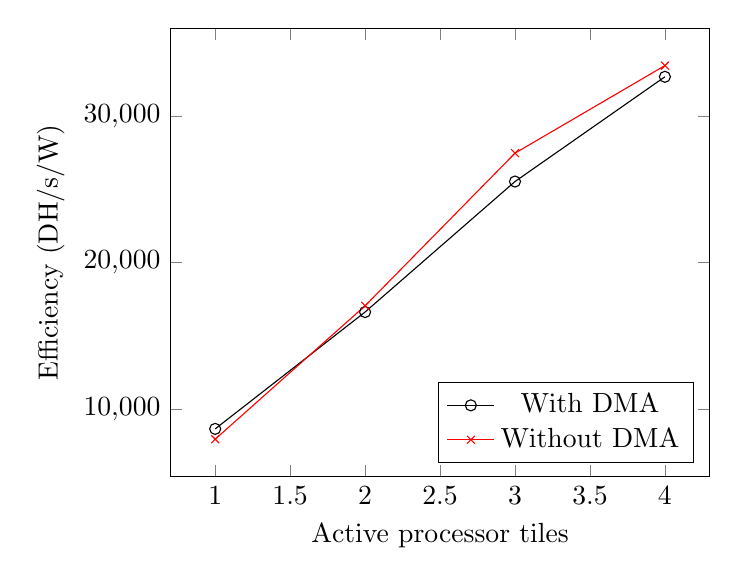
\begin{tikzpicture}
		\begin{axis}[
			xlabel=Active processor tiles,
			ylabel=Efficiency (DH/s/W),
			legend pos=south east,
			scaled ticks=false]
		\addplot[color=black,mark=o] coordinates {
			(1, 8681)
			(2, 16637.8)
			(3, 25522.7)
			(4, 32654.5)
		};
		\addlegendentry{With DMA}
		\addplot[color=red,mark=x] coordinates {
			(1, 7980.4)
			(2, 17063.2)
			(3, 27456)
			(4, 33418.6)
		};
		\addlegendentry{Without DMA}
		\end{axis}
	\end{tikzpicture}
	\caption{Energy efficiency when using hardware accelerators in the initial architecture.}
	\label{fig:SHADMA-eff1}
\end{figure}

%\subsection{Comparison, efficiency on 5x4 architecture}
%
%Surprisingly enough, when vomparing software hashing with SHA-256 accelerator hashing on the 5x4 architecture, greater energy efficiency can be achieved with software hashing when using 11 or 15 tiles.
%It is possible that this result is due to mere fluctuation in the power measurement, giving us a positive result, but constraining the use of SHA-256 accelerator to only up to four tiles puts great limit on the possible amount of double hashes.
%Given the near-linear scaling measured, the system could have achieved a much greater number of double hashes per second if it weren't for the constraint, with the possibility of out-performing the efficiency of software hashing by far. 
%
%\begin{figure}
%	\begin{tikzpicture}
%		\begin{axis}[
%			xlabel=Active processor tiles,
%			ylabel=Efficiency (H/s/W),
%			scaled ticks=false]
%		\addplot[color=red,mark=x] coordinates {
%			(1, 2804.3)
%			(2, 5372.9)
%			(3, 7995.8)
%			(4, 21261)
%			(5, 27585.7)
%			(6, 22985)
%			(7, 26092.9)
%			(8, 30318.3)
%			(9, 30325)
%			(10, 30320)
%			(11, 30323.3)
%			(12, 36384)
%			(13, 30320)
%			(14, 30318.3)
%			(15, 25987.1)
%			(16, 36382)
%		};
%		\addplot[color=black,mark=o] coordinates {
%			(1, 7980.4)
%			(2, 17063.2)
%			(3, 27456)
%			(4, 33418.6)
%		};
%		\addplot[color=blue,mark=x] coordinates {
%			(1, 8681)
%			(2, 16637.8)
%			(3, 25522.7)
%			(4, 32654.5)
%		};
%		\end{axis}
%	\end{tikzpicture}
%	\caption{Efficiency, Red: Software hashing. Black: SHA-256 accelerator (no DMA). Blue: SHA-256 + DMA. 5x4 architecture}
%	\label{fig:All-eff1}
%\end{figure}

\subsection{Alternative Architecture}

Table \ref{tab:SW-eff2} shows the energy efficiency of doing software hasing in the alternative architecture. The numbers
are plotted in figure \ref{fig:SW-eff2}. While performance is greates with only 4 tiles, the reduction in power usage
makes using of more tiles more efficient. 

\begin{table}
\centering
\begin{tabular}{| l | r | r || r |}
  \hline 
  \textbf{Cores} & \textbf{H/s} & \textbf{W} & \textbf{H/s/W} \\
  \hline                       
  \textbf{1} &  6418 & 2,3 & 2790.4\\
  \textbf{2} &  12841 & 2,5 & 5136.4\\
  \textbf{3} &  19130 & 2,3 & 8317.4\\
  \textbf{4} &  21364 & 1.0 & 21364\\
  \textbf{5} &  19404 & 0.9 & 21560\\
  \textbf{6} &  18420 & 0.8 & 23025\\
  \textbf{7} &  18253 & 0.8 & 22816.3\\
  \textbf{8} &  18206 & 0.8 & 22757.5\\
  \textbf{9} &  18193 & 0.7 & 25990\\
  \textbf{10} &  18192 & 0.7 & 25988.6\\
  \textbf{11} &  18192 & 0.8 & 22740\\
  \textbf{12} &  18192 & 0.8 & 22740\\
  \textbf{13} &  18191 & 0.7 & 25987.1\\
  \textbf{14} &  18190 & 0.7 & 25985.7\\
  \hline 
\end{tabular}
\caption{Energy efficiency when using software hasing only for the alternative architecture.}
\label{tab:SW-eff2}
\end{table}

\begin{figure}
\centering
	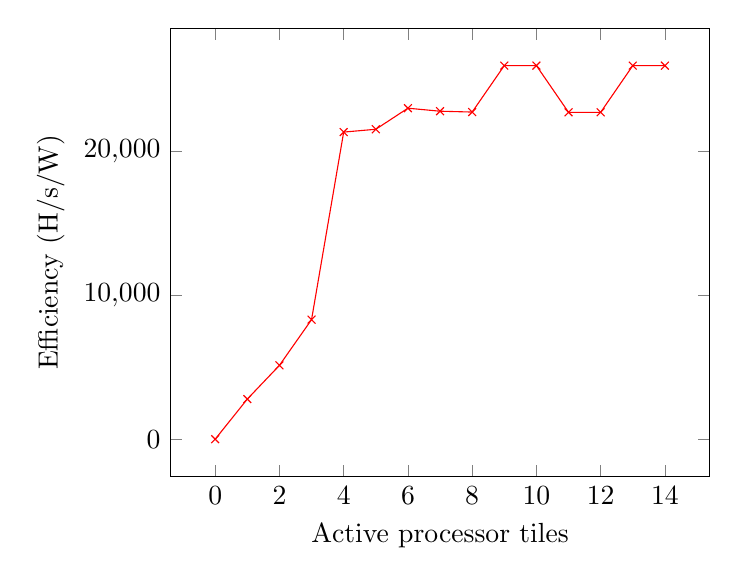
\begin{tikzpicture}
		\begin{axis}[
			xlabel=Active processor tiles,
			ylabel=Efficiency (H/s/W),
			scaled ticks=false]
		\addplot[color=red,mark=x] coordinates {
			(0, 0)
			(1, 2790.4)
			(2, 5136.4)
			(3, 8317.4)
			(4, 21364)
			(5, 21560)
			(6, 23025)
			(7, 22816.3)
			(8, 22757.5)
			(9, 25990)
			(10, 25988.6)
			(11, 22740)
			(12, 22740)
			(13, 25987.1)
			(14, 25985.7)
		};
		\end{axis}
	\end{tikzpicture}
	\caption{Energy efficiency when using software hashing only in the alternative architecture.}
	\label{fig:SW-eff2}
\end{figure}

Tables \ref{tab:SHA-eff2} and \ref{tab:SHADMA-eff2} shows the energy efficiency for the SHA-256 accelerator, without and with DMA module respectively.
%The numbers are plotted and compared in figure \ref{fig:SHADMA-eff2}.
%With the full scaling up to 14 tiles, it becomes much more clear that the use of DMA does not scale as well as without.
%Not is the poor performance of the SHA-256 + DMA usage the only reason, but using the DMA increases the power usage as well.
%It is clear that the system is more efficient when omitting the DMA Module, by up to 150\%, when all tiles become active.

\begin{table}
\centering
\begin{tabular}{| l | r | r || r |}
  \hline 
  \textbf{Cores} & \textbf{DH/s} & \textbf{W} & \textbf{DH/s/W} \\
  \hline                       
  \textbf{1} & 11676 & 2.1 & 5560\\
  \textbf{2} & 24394 & 2.1 & 11616.2\\
  \textbf{3} & 38329 & 2.1 & 18251.9\\
  \textbf{4} & 53760 & 2.1 & 25600\\
  \textbf{5} & 70983 & 2.1 & 33801.4\\
  \textbf{6} & 90590 & 2.1 & 43138.1\\
  \textbf{7} & 107510 & 2 & 53755\\
  \textbf{8} & 122186 & 1.9 & 64308.4\\
  \textbf{9} & 135009 & 1.8 & 75005\\
  \textbf{10} & 146221 & 1.6 & 91388.1\\
  \textbf{11} & 156133 & 1.6 & 97583.1\\
  \textbf{12} & 164860 & 1.5 & 109906.7\\
  \textbf{13} & 172381 & 1.3 & 132600.8\\
  \textbf{14} & 179526 & 1.1 & 163205.5\\
  \hline 
\end{tabular}
\caption{Energy efficiency using the SHA-256 accelerator for the alternative architecture.}
\label{tab:SHA-eff2}
\end{table}

\begin{table}
\centering
\begin{tabular}{| l | r | r || r |}
  \hline 
  \textbf{Cores} & \textbf{DH/s} & \textbf{W} & \textbf{DH/s/W} \\
  \hline                       
  \textbf{1} & 13227 & 2.2 & 6012.3\\
  \textbf{2} & 27410 & 2.4 & 11420.8\\
  \textbf{3} & 42627 & 2.3 & 18533.5\\
  \textbf{4} & 58989 & 2.4 & 24578.8\\
  \textbf{5} & 76556 & 2,4 & 31898.3\\
  \textbf{6} & 95259 & 2.4 & 39691.3\\
  \textbf{7} & 112599 & 2.3 & 48956.1\\
  \textbf{8} & 127515 & 2.2 & 57961.4\\
  \textbf{9} & 139937 & 1.9 & 73651.1\\
  \textbf{10} & 150069 & 2 & 75034.5\\
  \textbf{11} & 158421 & 1.9 & 83379.5\\
  \textbf{12} & 165271 & 2 & 82635.5\\
  \textbf{13} & 171143 & 1.9 & 90075.3\\
  \textbf{14} & 175711 & 1.7 & 103359.4\\
  \hline 
\end{tabular}
\caption{Energy efficiency using the SHA-256 accelerator with DMA for the alternative architecture.}
\label{tab:SHADMA-eff2}
\end{table}

%\section{Final notes}
%\todo{Yep}\textbf{Optional, if we need to note something extra. Remove if proven unnecessary}
%
%Reminder: DMA modules have four times the individual transfers, compared to CPU. Saturates the interconnect network faster.
%
% %***NOTE: not correct, for normal data transfers the CPU also does 32-bit transfers. Only for cache line loads does the CPU do 128 bit transfers.
%
%128-bit transfers would have increased efficiency greatly, by acting four times faster, and reduced traffic on the network.

\end{appendix}

